\documentclass{llncs}
\usepackage[utf8]{inputenc}
\usepackage[english]{babel}
\usepackage{hyperref}

\pagestyle{plain}

\newcommand{\liquidsoap}{Liquidsoap}
\newcommand{\savonet}{Savonet}
\newcommand{\eg}{e.g.~}
\newcommand{\cf}{cf.~}
\newcommand{\TODO}[1]{\marginpar{#1}}

\usepackage{graphicx}
\usepackage{xypic}

\usepackage{tikz}
\usetikzlibrary{snakes}

\title{Design of a Modular Programming Language for Generating Multimedia Streams: Liquidsoap}
\author{David Baelde \and Romain Beauxis \and Samuel Mimram}

\hypersetup{
  pdftitle={\csname @title\endcsname},
  pdfauthor={David Baelde, Romain Beauxis and Samuel Mimram},
  unicode=true,
  colorlinks=true,
  linkcolor=black,
  citecolor=black,
  urlcolor=black
}

\begin{document}
\maketitle

% \section*{Introduction}
The widespread of broadband Internet access and digital media during the last
decade has attracted a lot of attention on their potential applications.
Classical devices from the analog era, such as television, radio broadcasting
and phone communications are being adapted to the digital world. Additionally,
whilst analog applications were mostly based on hardware implementations, their
digital counterpart often consist in software implementations, \eg{} hardware
PBX for phone communications being replaced by software like Asterisk and IP
phones. These software implementations usually offer much more flexibility and
modularity in their design.
% and allow updates, both for bugfix and new features, at virtually no cost.

In this context of improvements, updates and enhancements of old technologies,
we are here specifically interested in adapting audio and video broadcasting
techniques to the digital world. Creating and broadcasting a stream of
multimedia data with recent computers has become technically very easy. However,
the software technologies available to perform such tasks have not yet brought
the new ideas which are necessary in order to benefit from the new possibilities
offered by modern computing devices.

Designing a generator form multimedia streams needs a lot of flexibility in
order to be able to cope with most of the expectations and requirements of
users. For instance, a radio stream may have jingles announcing next coming
shows or commercials. It may also play those jingles at a regular interval of
time, between songs or on top of them. Also, a radio program may be composed of
automatic playlist for a certain period, \eg{} during the night, and live shows
during the day. Similarly, one may want to control and process the data before
broadcasting it to the public, performing tasks like
\begin{itemize}
 \item volume normalization,
 \item cross-fading between tracks, possibly parameterized by the respective
   volumes of the old and new tracks or predefined settings,
 \item remove blanks, either in automatic file streams or during live shows,
 \item etc.
\end{itemize}

Those examples, among many others, show the need for very flexible and
adaptative solutions for creating and broadcasting multimedia data. Classical
tools to broadcast multimedia data over the Internet (such as Darkice, Ezstream,
VideoLAN, Rivendell or SAM Broadcaster) mostly consist of straightforward
adaptation of classical streaming technologies, whose paradigms are based on
predefined interfaces, such as a virtual mixing console or static file-based
setups. Those tools, although quite powerful, are usually very hard to adapt to
a particular need and are more and more often perceived as limited by the very
constrained design of the program.

A particularly important aspect of modern software technologies is programming
languages. Whether general or applicative, programming languages are the first 
class tools to release creativity and flexibility for creating new software applications.
Programming languages have been used in various practical contexts to bring flexibility
and overcome static pre-defined paradigms. One may, for instance, think of the Perl 
language, invented to allow powerful and flexible word-based treatments, or the PHP
language, invented to create easily dynamic web pages.

The application we present in this paper brings to the domain of multimedia
broadcasting the ideas and technologies of software engineering. It originated 
after realizing that the existing tools for digital broadcasting where not flexible
and expressive enough to fit the authors' need. In order to overcome those shortcomings,
an applied language was developed which, as for Perl and PHP, includes first-class
notions of streams, with operators to create them, combine them and modify them.
Using this language, the possibilities for designing and creating a multimedia stream
are very broad and allow creative innovations.

Another important aspect of this application is its potential users. Multimedia stream 
designers are not often programming language specialists. Moreover, creating an Internet 
radio should not require advanced programming skills.
For there reasons, although the language is intended to be powerful, it should 
also be relatively easy to use, at least for building a basic stream.

The language, called \liquidsoap{} \cite{liquidsoap}, is a functional language, implemented as 
a script language, with an interpreter written in OCaml. In the following,
we present the model that was used to build multimedia streams, then
the language that implement it, show some of its applications and explain the 
related theoretical interesting considerations.
TODO: expand this part when we know what we are talking about :-)

TODO: somehow described in~\cite{baelde-mimram:webradio-lambda}

TODO: has been used in research~\cite{baccigalupo2007case,baccigalupo2007sharing}.

\section{A model for describing streams}
\TODO{arbre (partage), transitions (partage plus compliqué, activations dynamiques), clocks (boites);}

A multimedia stream can be understood as a timed sequence of data. For instance, a sequence of songs with
track marks and metadata information, or a live input, encoded real-time from the sound card.

\begin{figure}[htn]
 \begin{center}
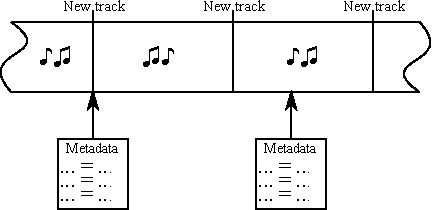
\includegraphics{stream}
\end{center}
 \caption{A \liquidsoap{} stream}
 % Stream.png: 500x132 pixel, 91dpi, 14.03x3.70 cm, bb=0 0 398 105
\end{figure}

The timing, or clock, associated to a multimedia stream can be real-time, if the stream is created 
or broadcasted live, or any scaled timing, for instance if the stream consists of files. \textit{A priori},
describing and broadcasting a stream implies real-time output. As we see later, this is unfortunately 
not sufficient for complex settings.
Also, a stream can be finite or infinite. Infinite streams are particularly interesting for broadcasting
because most of the time, we expect a radio, for instance, to be always online. However, this needs 
a special care since it implies some assumption about the validity of the elements that build the stream.

Because stream are infinite objects, they cannot be fully instantiated in memory. Hence, it is 
more appropriate to think of a \textit{stream generator} than of a stream itself which is how
a stream is created in \liquidsoap{}. A stream generator, in \liquidsoap{}, is described as 
an acyclic oriented graph. The edge of the graphs represent the operators, used to create and modify
a stream, while the vertices represent the connections between them.

\subsection*{Stream generation}

Given an acyclic graph describing a stream generator, the roots of the graph are the operator that create 
the initial streams, called \textit{sources}. Those sources can be create from a single file, a playlist, an HTTP input,
the sound card, etc.. The sources are then modified and composed with each other using 
\textit{operators} that, for instance, play a source if it is available or a second one otherwise, or modify
the metadata, mix the audio data of two sources, etc..
Finally, the leaves of the graph describe the \textit{outputs} of the stream. Those outputs consist, for instance,
of playing the stream on the local sound card, saving it to a file or sending it to and Icecast server. 
For this initial description, we suppose that the graph has only one output.

As explained, the graph is a \textit{stream generator}. Hence, once the graph has been instantiated,
it is used to generate the stream in the following way: a elementary chunk of data, called a frame, is given to be filled to the 
output operator, the leave of the graph, assumed to be unique for now. 
The output passes the frame to the underlying operators to fill it. Those operators, in turns, pass the frame to their 
underlying operators, until the frame reaches a root node, i.e. a source. 
Then, the source fills the frame and send it back to the operator above, which in turn performs
the modifications it has to do, until a filled frame is returned to the output.

\begin{figure}[htn]
 \begin{center}
\[
\xymatrix{
  *+[F]{\mathtt{input.http}}\ar[r]&*+[F]{\mathtt{fallback}}\ar[r]&
  *+[F]{\mathtt{normalize}}\ar[r]&
  *+[F]{\mathtt{output.icecast}}\\
  *+[F]{\mathtt{playlist}}\ar[ur]&\\
}
\]
\end{center}
 \caption{A stream generator}
 % Stream.png: 500x132 pixel, 91dpi, 14.03x3.70 cm, bb=0 0 398 105
\end{figure}

Using this method, the stream can be described using a finite amount of memory. In fact, the frames used
to generate the stream can be statically allocated and passed as memory pointers during the generation, which 
avoids copying data in memory. Also, the stream generator can be used at any rate. For instance,
for a live broadcast, the generator will be asked to fill frames at real rate, while 
for a stream saved to a file, the generator will be asked to fill frames at the maximal possible rate.

Finally, the information of whether or not a stream can be assumed to be infinite is also carried by the 
graph. For instance, if a source is created from a single file, one can try to decode it before starting 
streaming. If the file can be decoded, and one can assume that the file will not be deleted later, and then 
the source can be considered infallible. Later one, if this source is used, for instance in an operator that plays 
the first available source, then the source resulting of this operator is also infallible etc..
By induction over the vertices of the graph, each node can be considered fallible or not. Eventually,
an infallible output can be considered as describing an infinite stream, while a fallible
output describes a stream that may not be infinite.

\subsection*{Stream sharing}

The description of a stream generator in the previous section is neat. Unfortunately, most 
of the time it is too limited. For instance, one may want to have several output of the same 
stream, one to a local file for archiving purposes and another one to an Icecast server to be
broadcasted.
In this case, the two output in the graph are connected to the same operator. Hence, when those output
transmit their frame to this operator to be filled, the operator should fill them with the same data.

\begin{figure}[htn]
 \begin{center}
\[
\xymatrix{
  *+[F]{\mathtt{input.http}}\ar[r]&*+[F]{\mathtt{fallback}}\ar[r]&
  *+[F]{\mathtt{normalize}}\ar[r]\ar[dr]&
  *+[F]{\mathtt{output.icecast}}\\
  *+[F]{\mathtt{playlist}}\ar[ur]& & & *+[F]{\mathtt{output.file}}\\
}
\]
\end{center}
 \caption{A stream generator with caching}
 % Stream.png: 500x132 pixel, 91dpi, 14.03x3.70 cm, bb=0 0 398 105
\end{figure}


For this reason, the first time that the operator is asked to fill the frame, it should pass it to its 
underlying operators, as described before. However, the second time, it should just fill the frame 
with the data gathered during the first call, which implies \textit{caching} the data obtained during the first call.

Therefore, even though the initial stream generator model could avoid copying data in memory, there 
are situations where it is not possible. In order to deal with these situations, the 
model carries a notion of \textit{ticks}. Ticks represent an elementary unit of time
for stream generation. Each frame contains a fixed number of ticks and the stream is split
in bunches of ticks representing each frame. During the same bunch of ticks, when filling a frame, the nodes only 
transmit their frame to their underlying nodes once and, for the successive calls, use a cache of this data. 
Once all the filling operations have been done for a bunch of ticks, the nodes are informed that the 
stream has moved to the next bunch and reset their cached values. 

Finally, the necessity for a node to cache its current frame is detected when instantiating the graph, thus
copying data in memory only when it is necessary.

\subsection*{Stream clocks}

Another limitation of the current model is the possibility to describe advanced transitions in 
the stream. For instance, one may want to use a crossfade between two tracks of the stream, i.e.
fade out the volume of an ending track, fade in the volume of a starting track and merge this together.

\begin{figure}[htn]
 \begin{center}
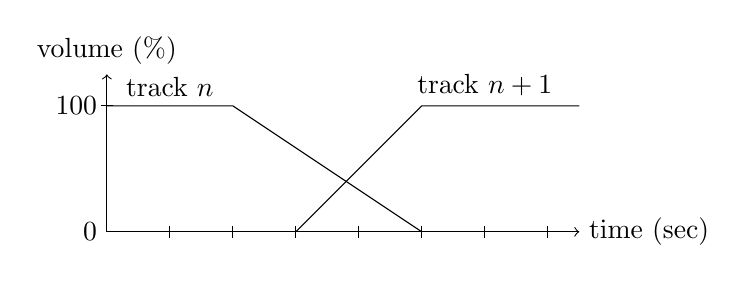
\begin{tikzpicture}[xscale=0.8,yscale=0.8]
\draw[->] (0,0) -- (0,2.5);
\draw (-0.1,2) -- (0.1,2);
\draw (0,2) node[anchor=east]{100};
\draw (0,0) node[anchor=east]{0};
\draw[->] (0,0) -- (7.5,0);
\foreach \x in {1,2,3,4,5,6,7} \draw (\x,-0.1) -- (\x,0.1);
\draw (0,2.5) node[anchor=south]{volume (\%)};
\draw (7.5,0) node[anchor=west]{time (sec)};
\draw (0,2) -- (2,2) -- (5,0);
\draw (3,0) -- (5,2) -- (7.5,2);
\draw (1,2) node[anchor=south]{track $n$};
\draw (6,2) node[anchor=south]{track $n+1$};
\end{tikzpicture}
\end{center}
 \caption{A crossfade transition between two tracks}
 \label{cross-fig}
 % Stream.png: 500x132 pixel, 91dpi, 14.03x3.70 cm, bb=0 0 398 105
\end{figure}

The initial source can be created, for instance, with a playlist of files. Then,
a \texttt{crossfade} operator would take this source and return a source whose tracks are 
crossfaded as shown in Figure \ref{cross-fig}. In order to do this, the operators has to 
detect sufficiently in advance the end of the current track, collect the data of the
end of the track, collect the data of the beginning of the next track, apply the respective
fade out and fade in and add the two streams to create the transition.

However, in this case we need to introduce a new notion in the model. Without transitions, the 
source generator can be used with a uniform rate on all nodes: frames are filled
at the same rate on every node. Unfortunately, the \texttt{crossfade} operator
does not have this property: when it detects the end of a track, it will query many frames in advance 
to the underlying source in order to compute the crossfade. This behaviour breaks the uniformity of 
timing in the graph and requires to introduce \textit{local clocks}.


\begin{figure}[htn]
 \begin{center}
\[
\def\f{\save
*+<15pt>[F--]\frm{}\ar @{--} "1,1"\restore}%
\def\g{\save
"2,4"."1,3"."1,5"!C*+<15pt>[F--]\frm{}\ar @{--} "2,2"\restore}%
\xymatrix{
   \mathtt{clock_1} & *+[F]{\mathtt{playlist}}\ar[r]\f&*+[F]{\mathtt{crossfade}}\ar[r]&  *+[F]{\mathtt{fallback}}\ar[r]&
  *+[F]{\mathtt{output.icecast}}\\
   &\mathtt{clock_2} &  & *+[F]{\mathtt{jingles}}\ar[u]\g& 
}
\]
\end{center}
 \caption{A stream generator with different clocks}
 % Stream.png: 500x132 pixel, 91dpi, 14.03x3.70 cm, bb=0 0 398 105
\end{figure}

Clocks are represented in the model by a notion of locality in the graph. The graph is then partitioned into 
different sets, where each set shares the same clock.
When instantiating the graph, each operator declares if it needs a custom clock for him or its sources. 
Then, when initializing the graph of the stream generator, the clocks are attributed by a constraint 
satisfaction algorithm. Because of caching, we do not want a source to be connected to two different operators with 
two different clocks. In this case, this is detected when instantiating the graph and an error is raised.
Similarly, some sources do not support clocks whose rate is different than real time, for instance input 
from the local sound card. In this case too, if the clock attached to the source is not real time, an error
is raised.



\section{The \liquidsoap{} language}
\label{sec:lang}

The \liquidsoap{} language is the formal tools developed to describe the graph of the
stream generator of our model.

\bibliographystyle{abbrv}
\bibliography{biblio}
\end{document}
